\documentclass[11pt,letterpaper]{exam}
\usepackage[utf8]{inputenc}
\usepackage[spanish]{babel}
\usepackage{graphicx}
\usepackage{tabularx}
\usepackage[absolute]{textpos} % Para poner una imagen en posiciones arbitrarias
\usepackage{multirow}
\usepackage{float}
\usepackage{hyperref}
\usepackage[utf8x]{inputenc} 
\usepackage[normalem]{ulem}
\useunder{\uline}{\ul}{}
\usepackage[usenames]{color}
\title{Tarea 2 Métodos Computacionales\\\\ Departamento de Física \\ Universidad de los Andes}
\author{Valeria Martín Hernández\\\\201631501}

\date{Mayo 2019}

\begin{document}
\maketitle
\newpage


\addcontentsline{}{}{}
\tableofcontents

\newpage


\section{Ejercicio 2: Transformadas de Fourier}
\subsection{Signal.dat y signalSuma.dat:}
\subsubsection{Grafica general}
\begin{figure}[H]
    \centering
    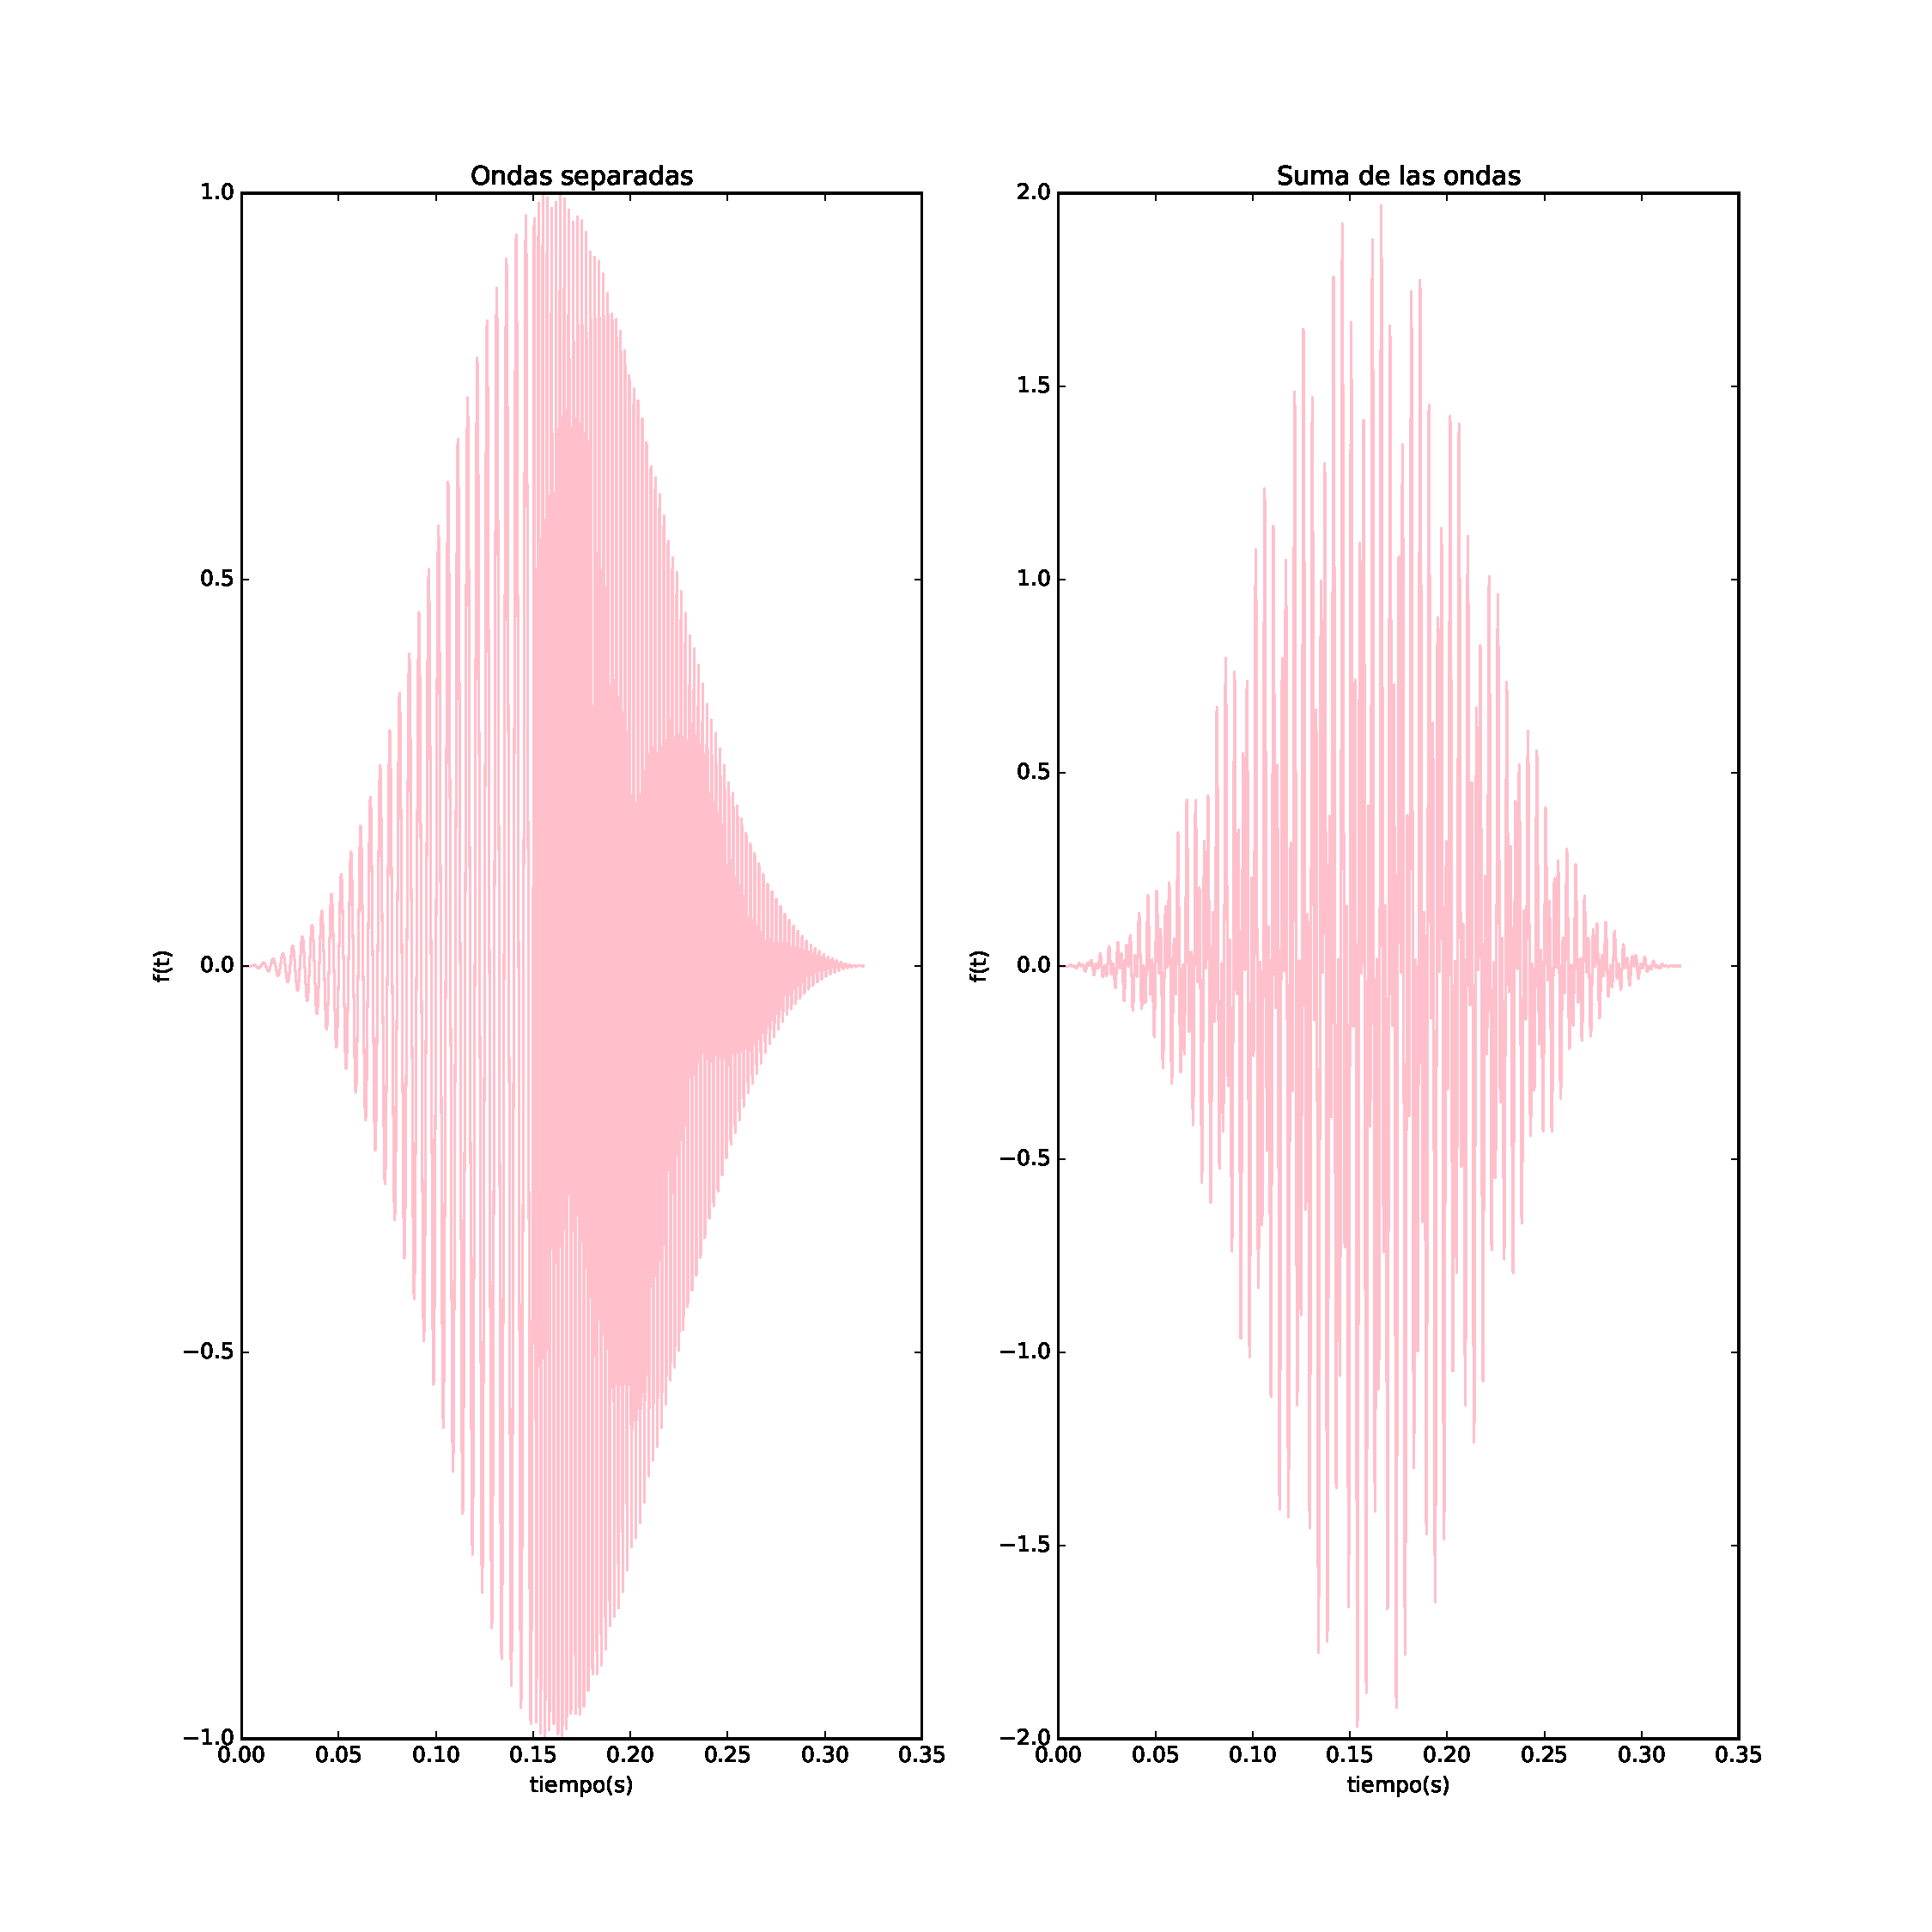
\includegraphics[width=1.1\textwidth]{signals.pdf}
    \caption{Grafica de las seniales.}
    \label{fig:my_label}
\end{figure}
\subsubsection{Grafica de la transforma de fourier para las seniales}
\begin{figure}[H]
    \centering
    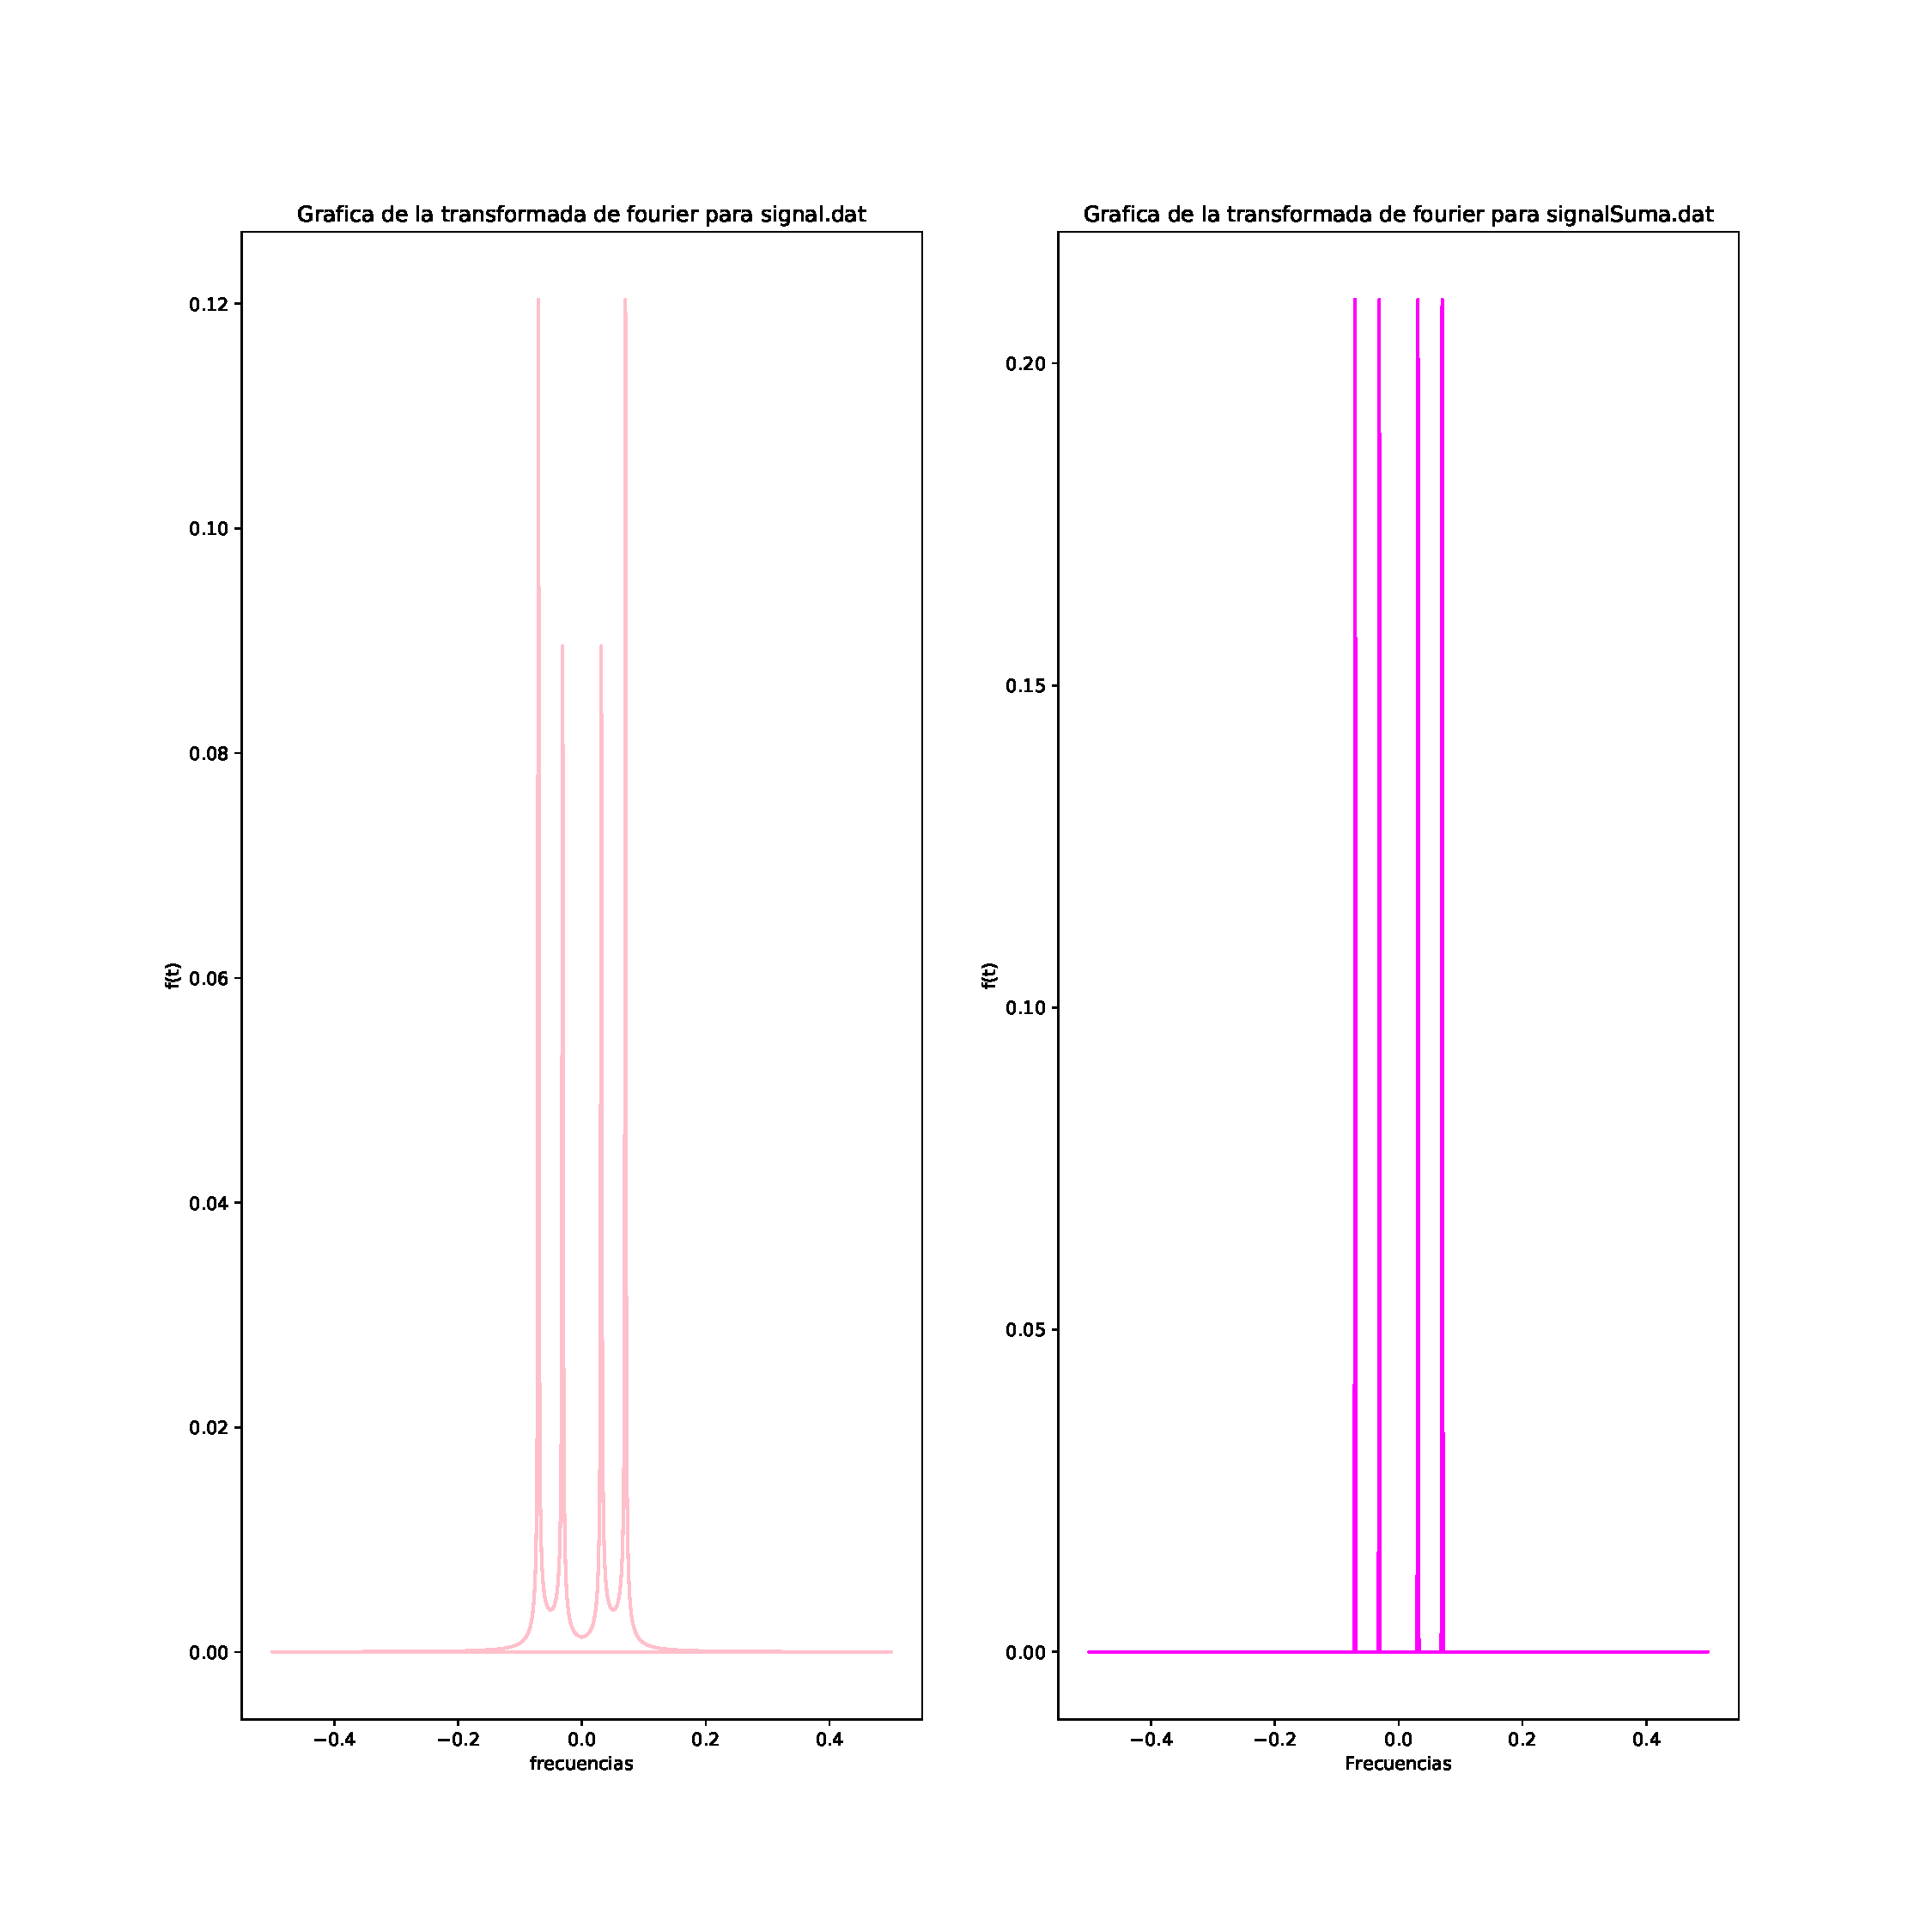
\includegraphics[width=1.1\textwidth]{Fourier_trans.pdf}
    \caption{Grafica de las transformadas de fourier para las dos primeras seniales.}
    \label{fig:my_label}
\end{figure}
\subsubsection{Espectograma}
\begin{figure}[H]
    \centering
    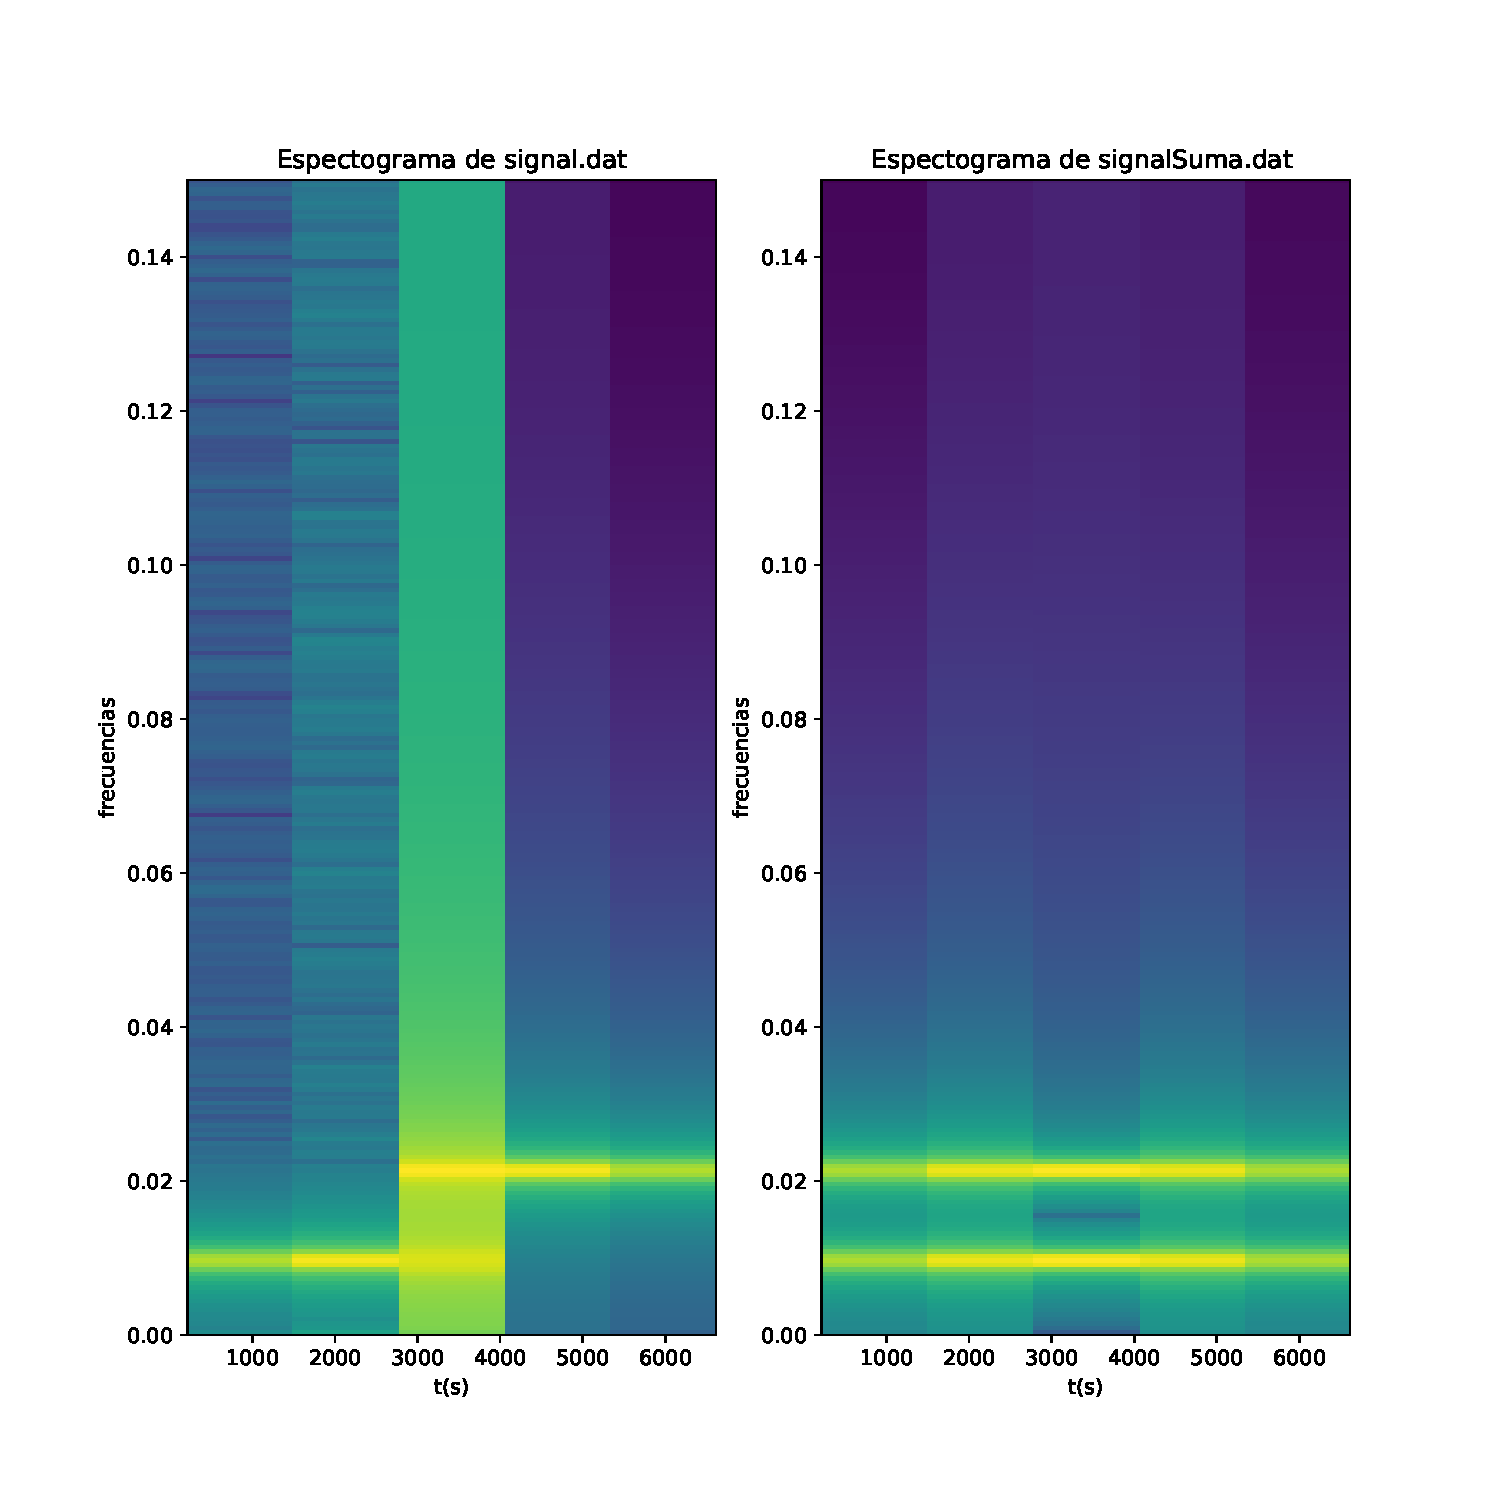
\includegraphics[width=1.1\textwidth]{espectograma.pdf}
    \caption{Espectogramas de las dos primeras seniales.}
    \label{fig:my_label}
\end{figure}
\subsection{Temblor.txt:}
\subsubsection{Grafica general}
\begin{figure}[H]
    \centering
    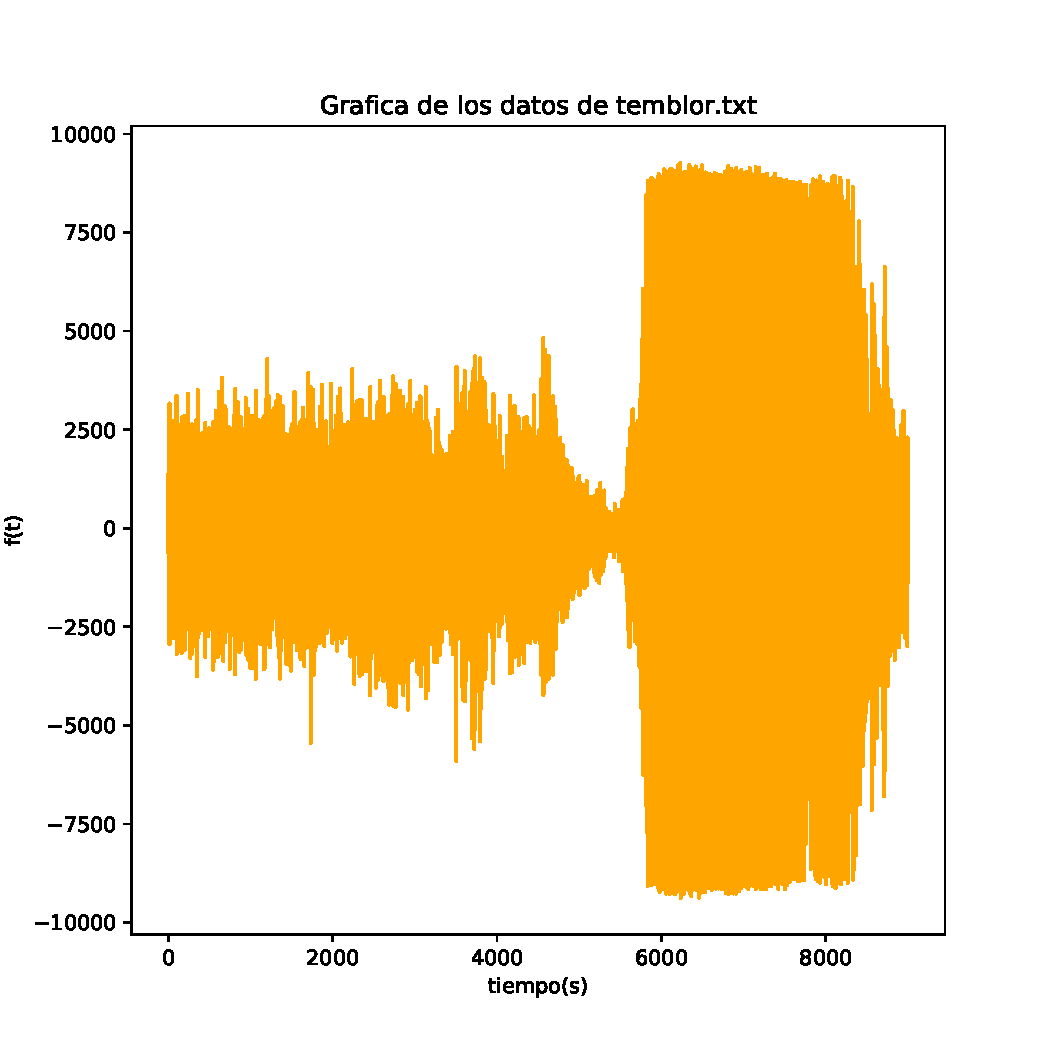
\includegraphics[width=1.1\textwidth]{Temblor.pdf}
    \caption{Grafica de los datos de temblor.txt}
    \label{fig:my_label}
\end{figure}
\subsubsection{Grafica transformada de fourier}
\begin{figure}[H]
    \centering
    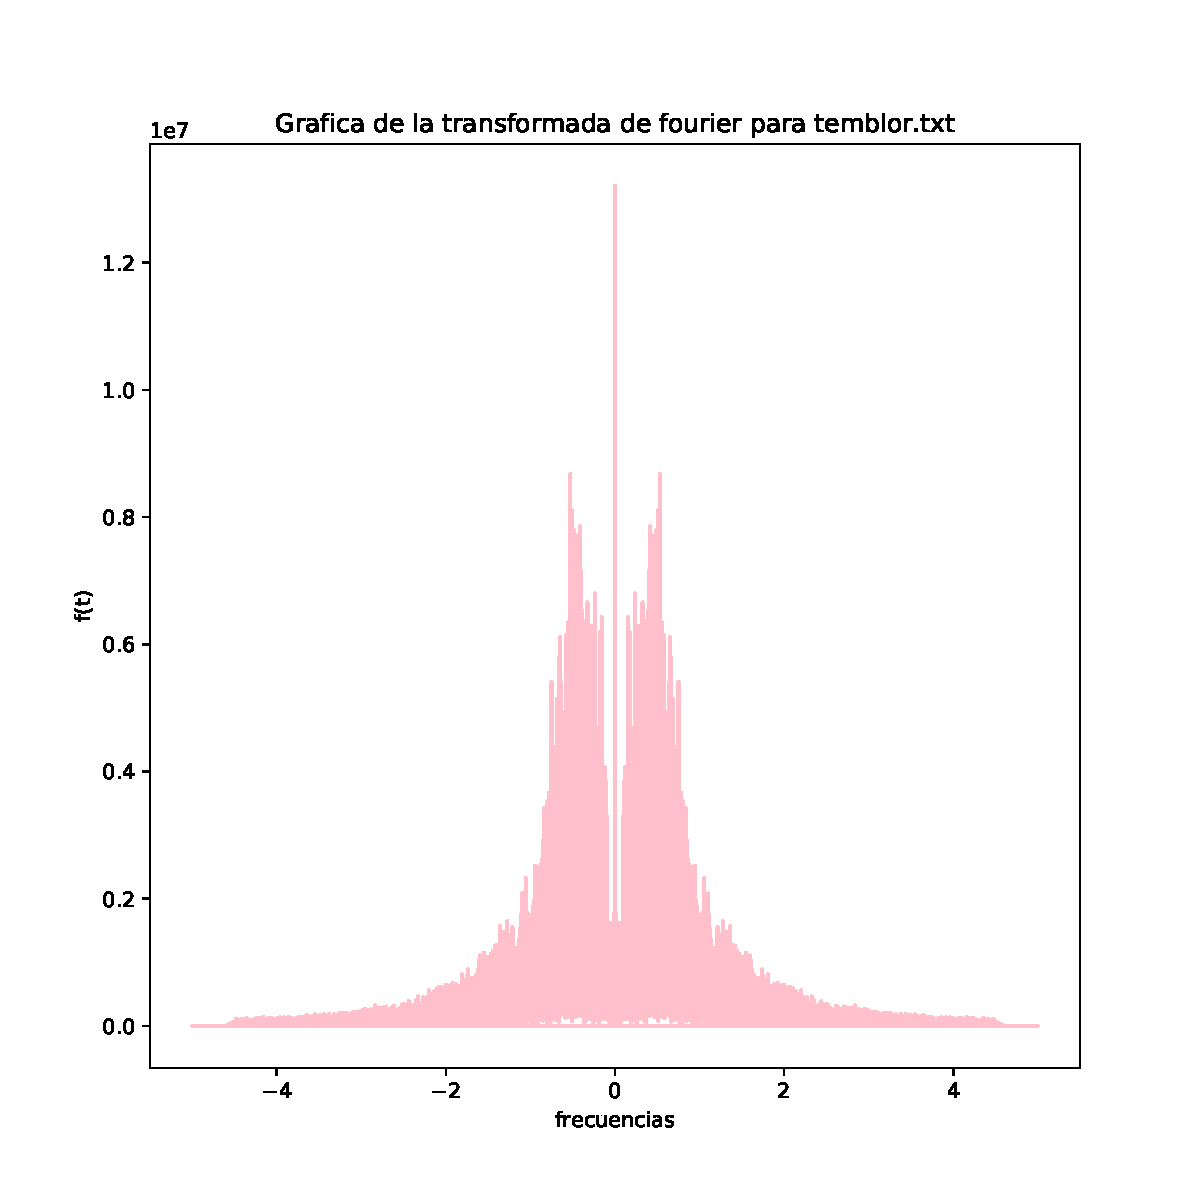
\includegraphics[width=1.1\textwidth]{Fourier_temblor.pdf}
    \caption{Grafica de las transformada de fourier de los datos de temblor.txt}
    \label{fig:my_label}

\end{figure}
\subsubsection{Espectograma}
\begin{figure}[H]
    \centering
    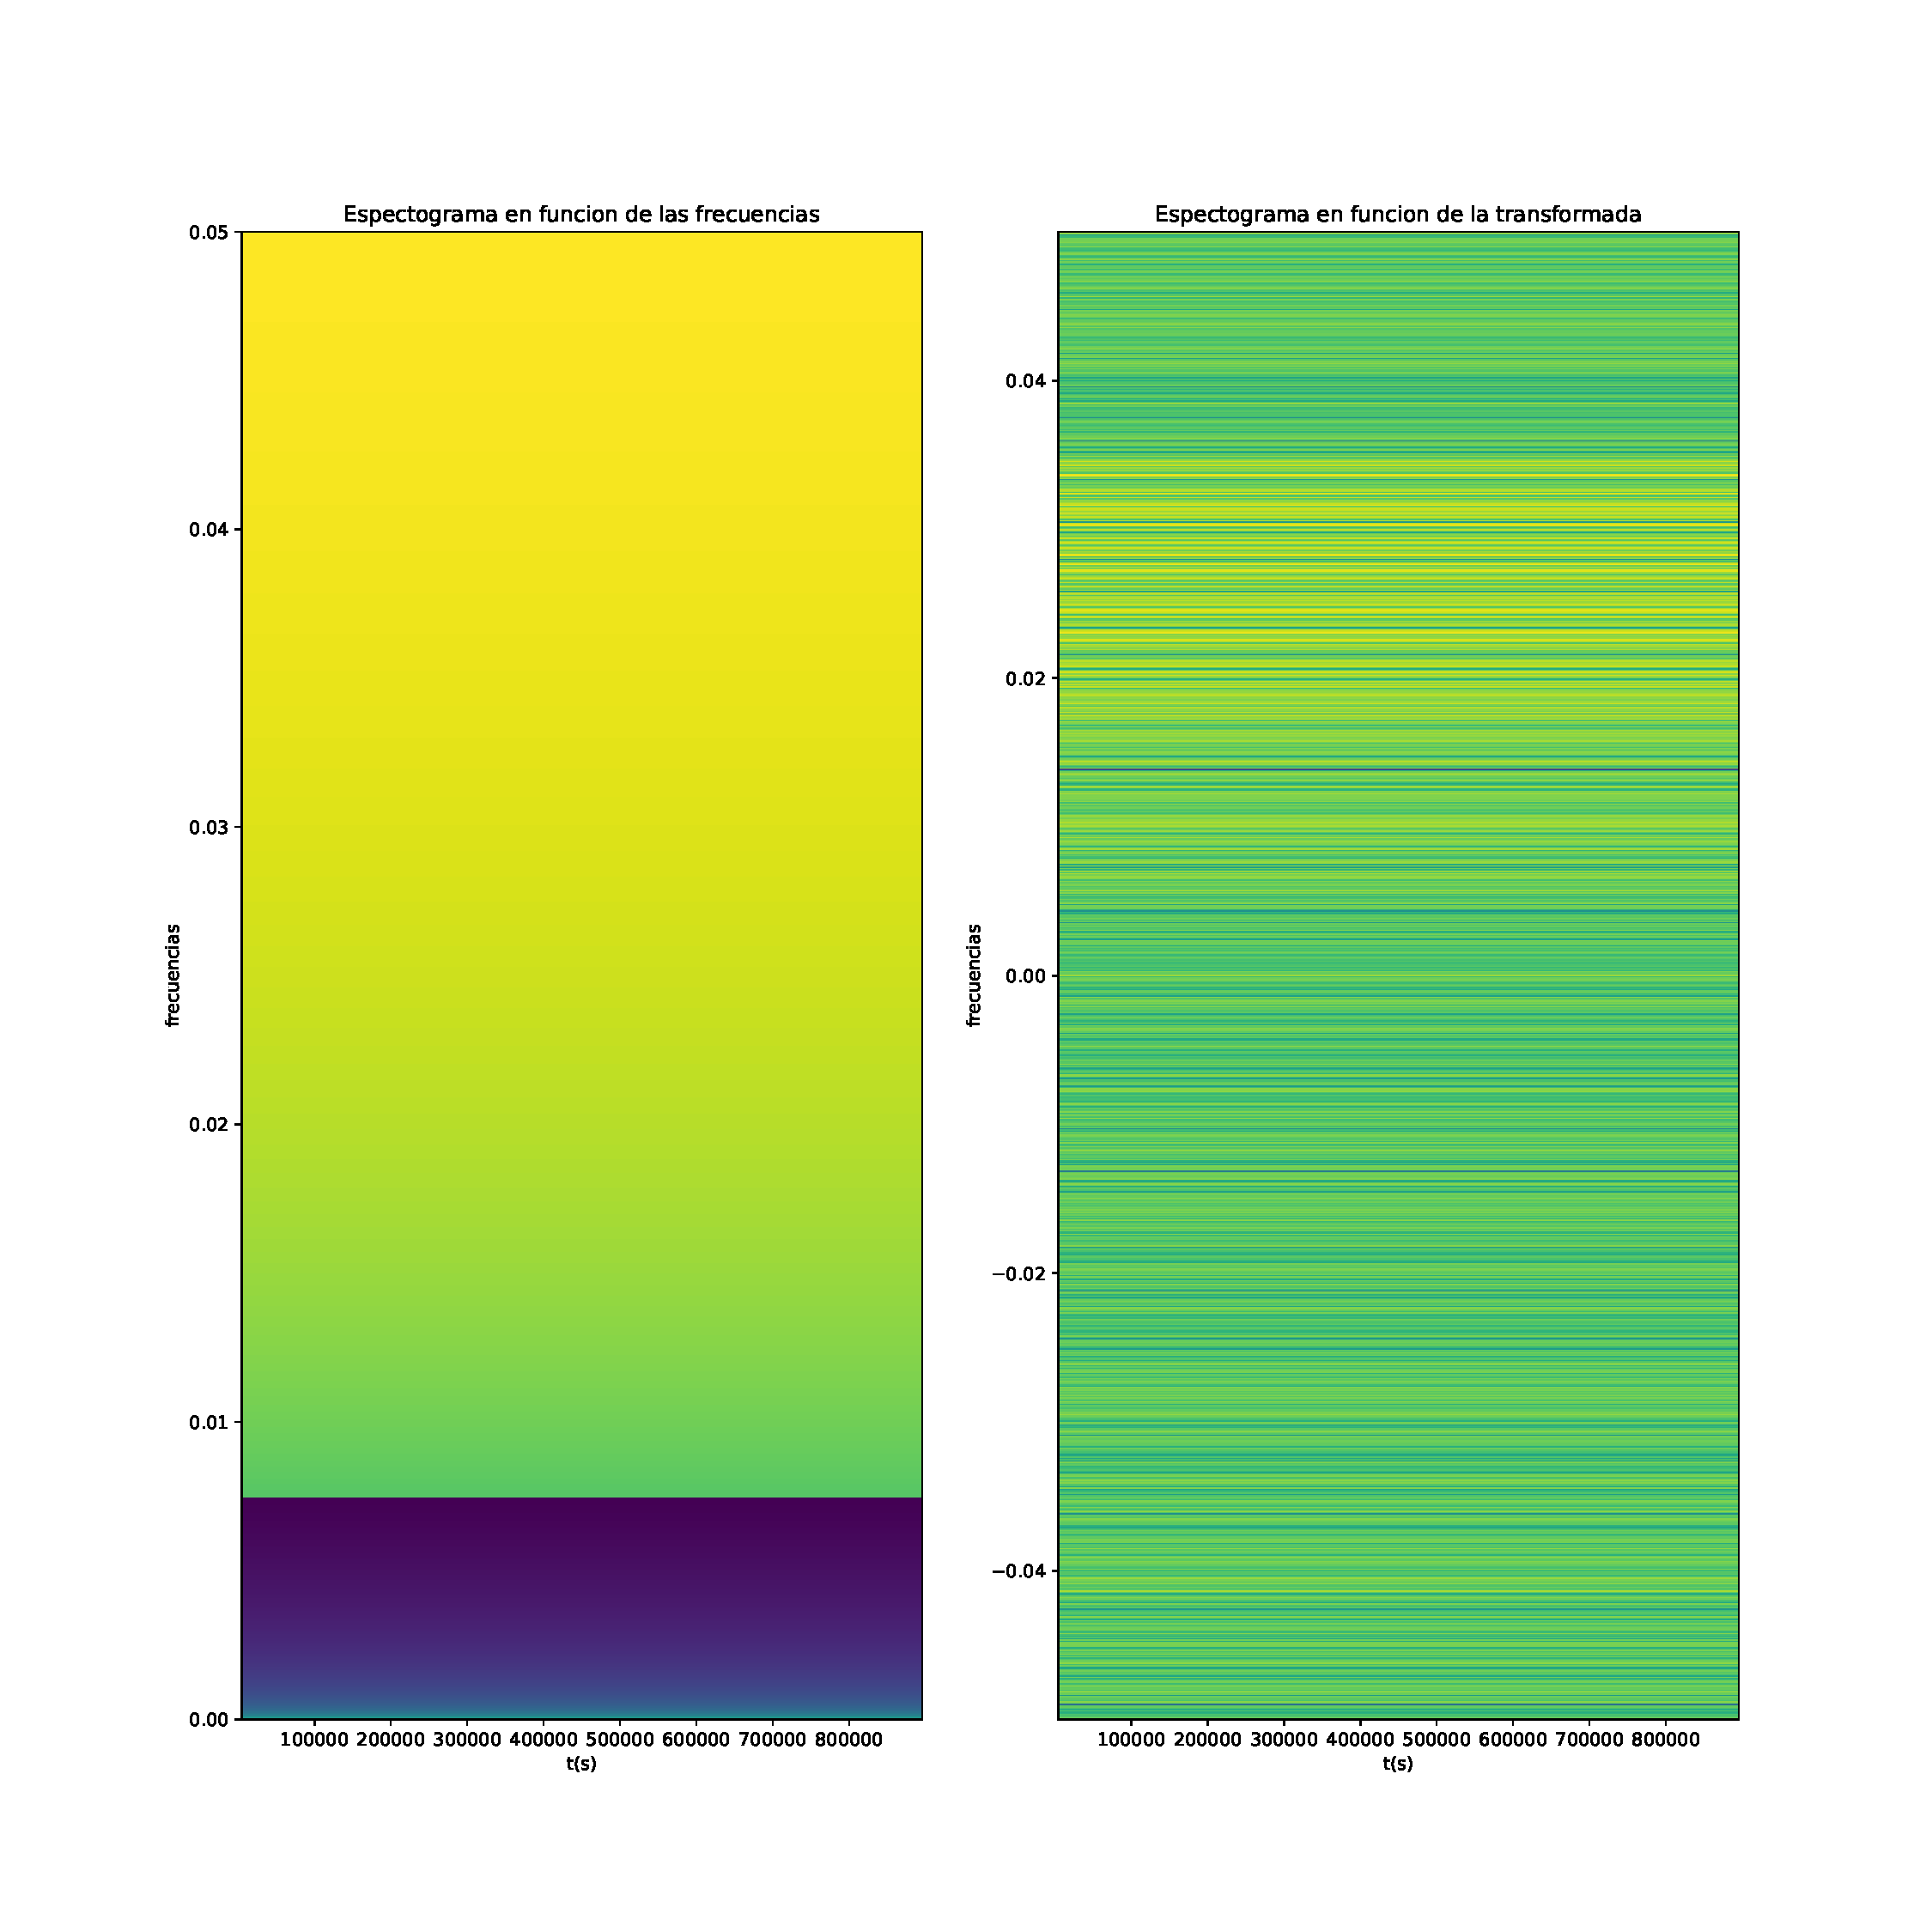
\includegraphics[width=1.1\textwidth]{espectograma_temblor.pdf}
    \caption{Espectograma del temblor}
    \label{fig:my_label}
\end{figure}
\section{Ejercicio 2: Ecuaciones diferenciales ordinarias}
\subsection{Primera grafica para $\omega$ = 1*$\sqrt{\frac{k}{m}}$}
\begin{figure}[H]
    \centering
    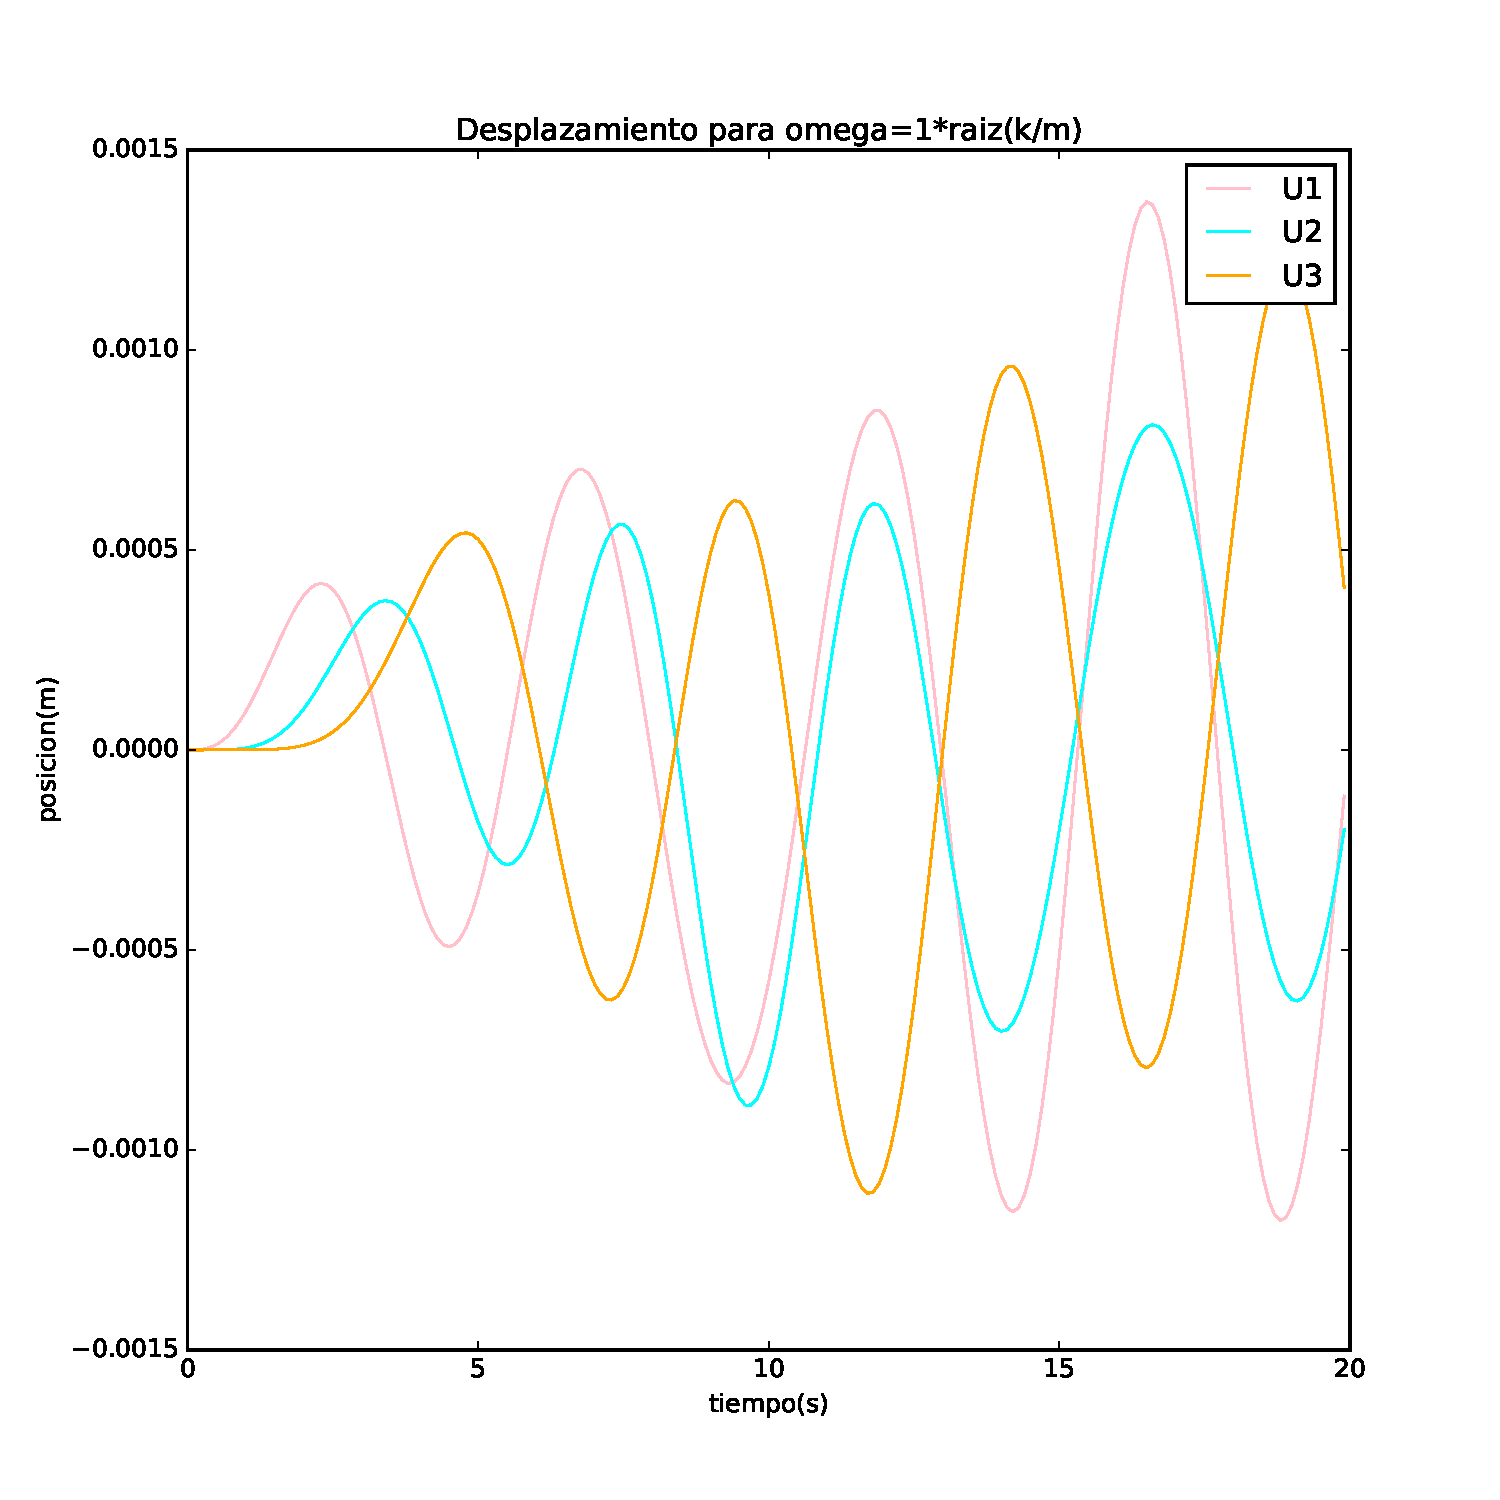
\includegraphics[width=1.1\textwidth]{plot_omegafijo.pdf}
    \caption{Desplazamiento del edificio en el tiempo}
    \label{fig:my_label}
\end{figure}
\subsection{Grafica de las mayores amplitudes para cada uno de los 100 omegas generados}
\begin{figure}[H]
    \centering
    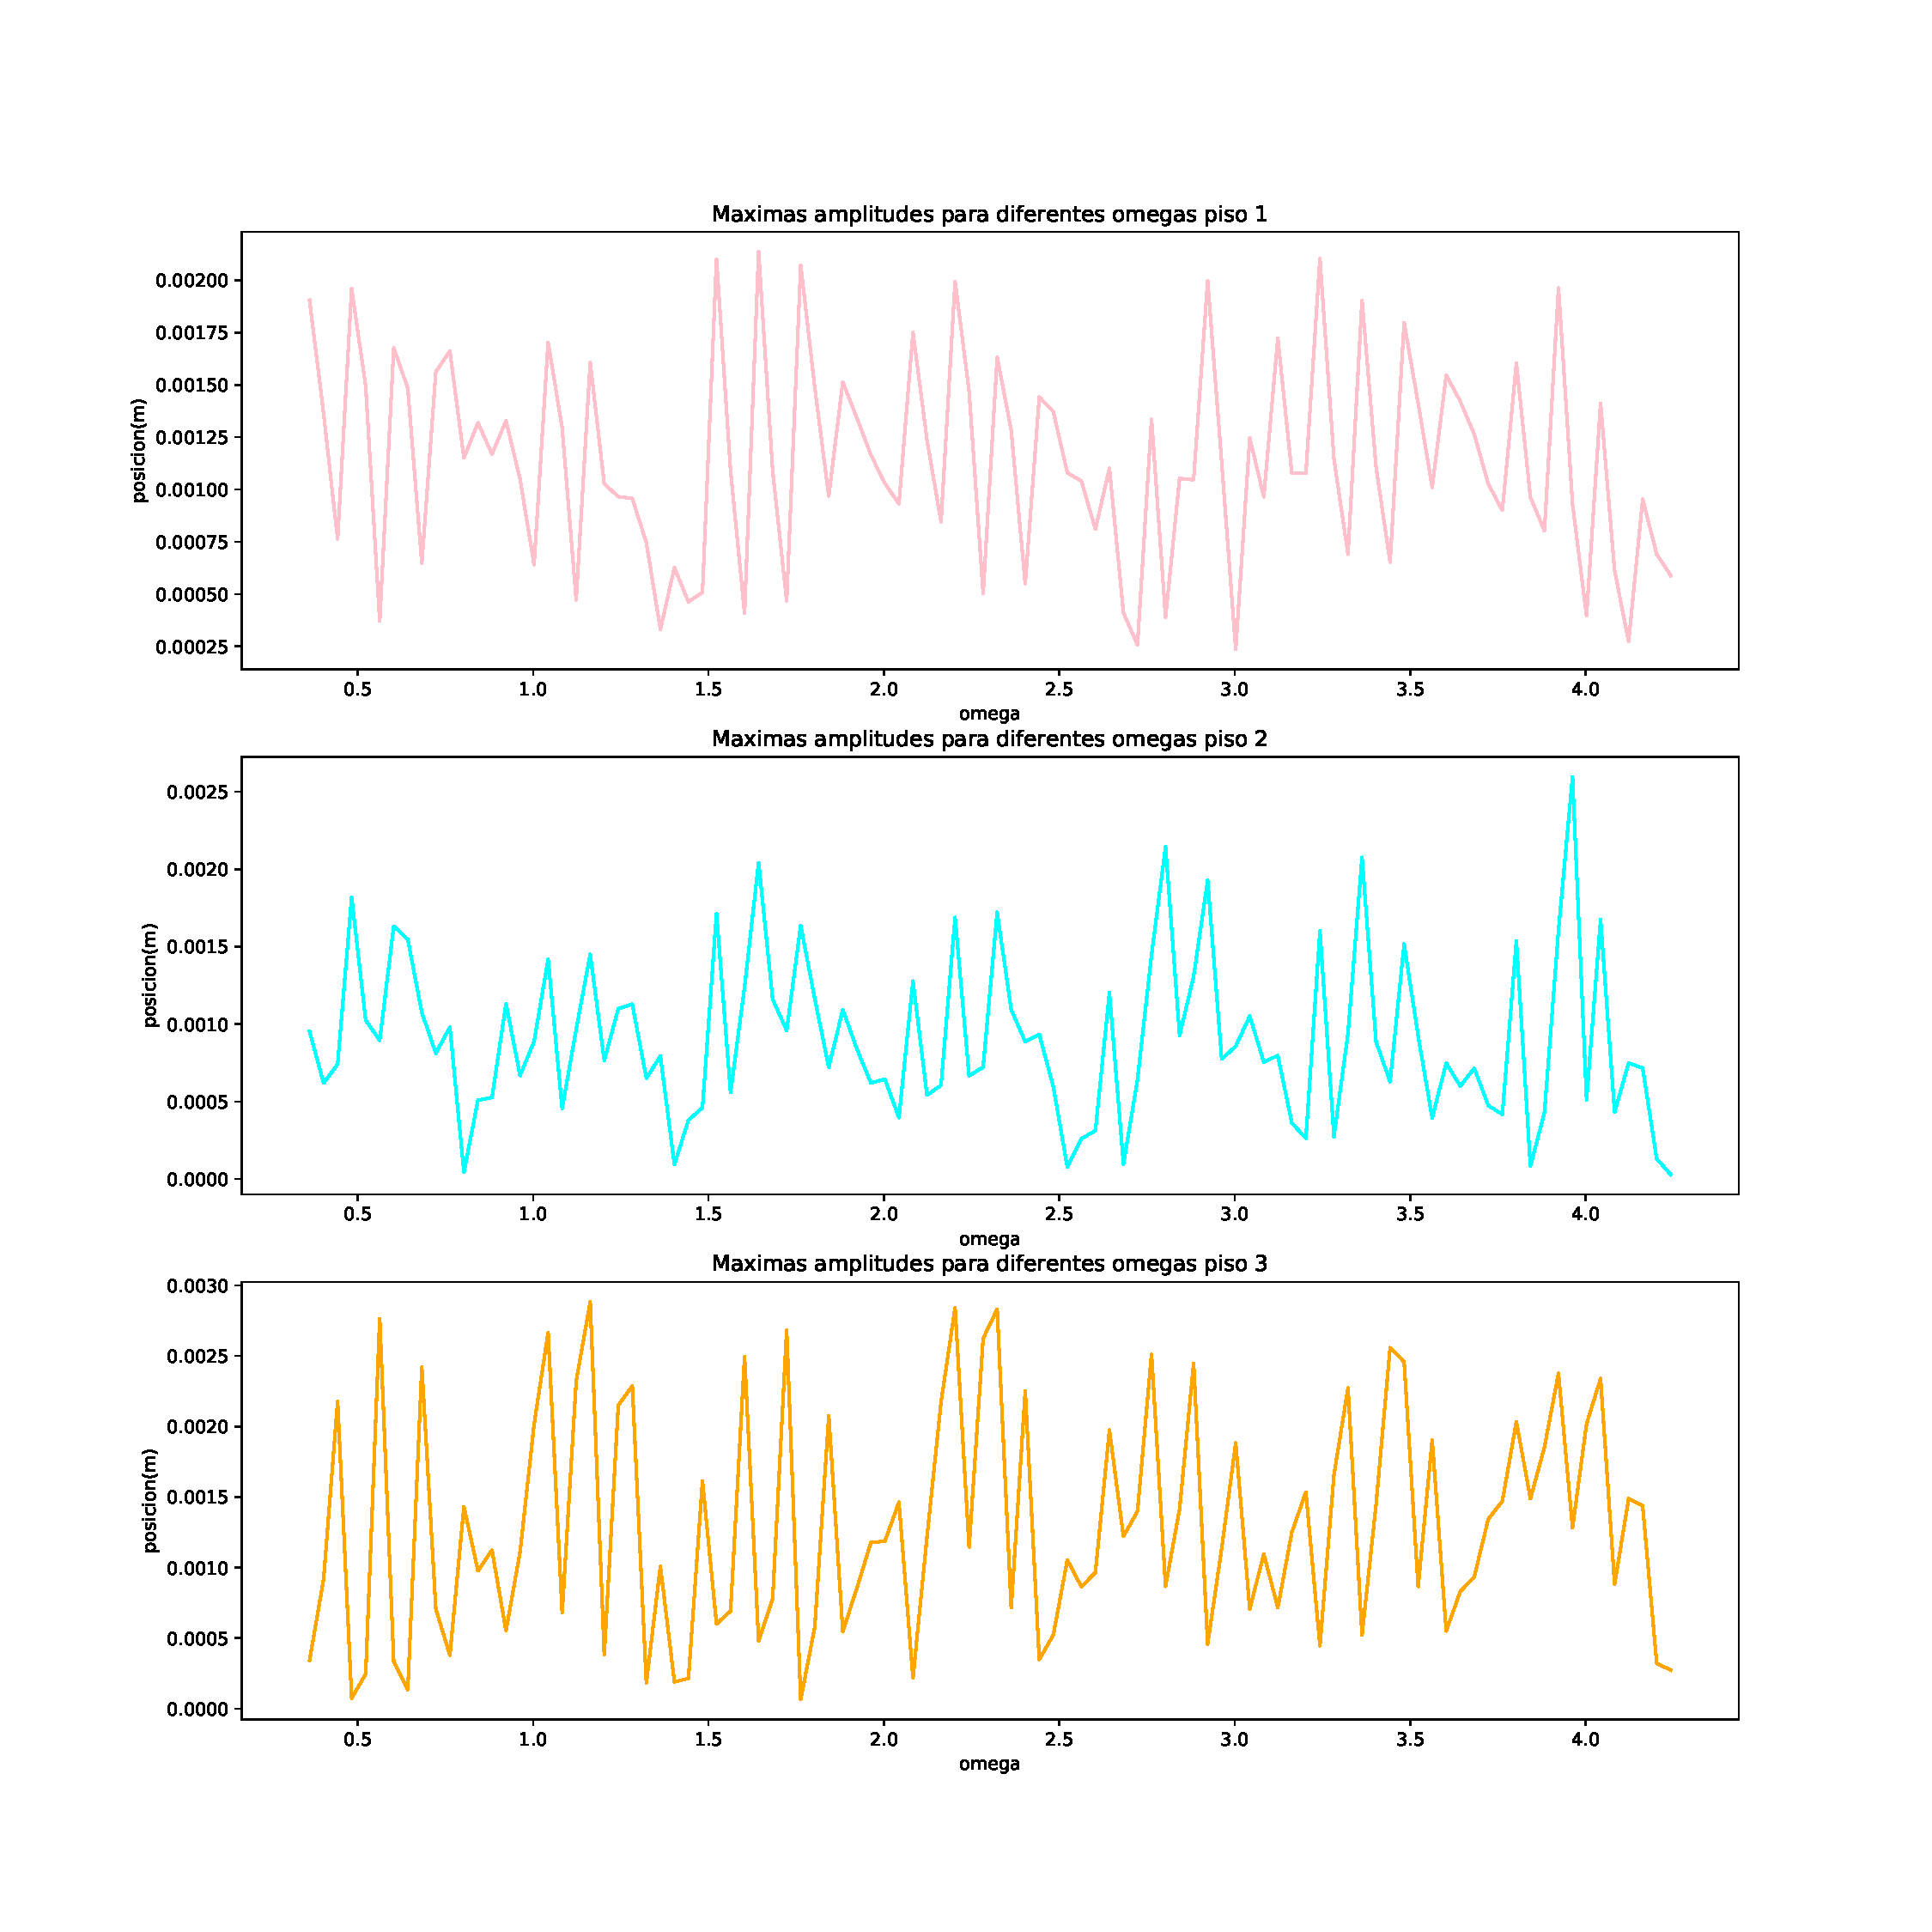
\includegraphics[width=1.1\textwidth]{plot_omegas.pdf}
    \caption{Mayores amplitudes para cada omega}
    \label{fig:my_label}
\end{figure}
\subsection{Grafica de los cuatro omegas}

\end{document}